\chapter{Evaluation}
\label{chap:Evaluation}

\section{Contexte}
Dans une tâche d'object detection, nous utilisons le score IoU qui signifie Intersection over Union.
C'est un score qui compare les bounding boxes prédites par le modèle avec les bounding boxes réels (ground-truth).
Une tâche d'object detection comprend deux sous-problèmes: la classification et la localisation.
Ainsi nous avons plusieurs métriques pour analyser la performance d'un modèle. IoU se concentre sur 
la localisation des bounding box prédites tandis que la métrique mAP (mean Average Precision) 
se concentre sur la classification.
\begin{figure}[bh!]
    \centering
    \scalebox{0.5}[0.5]{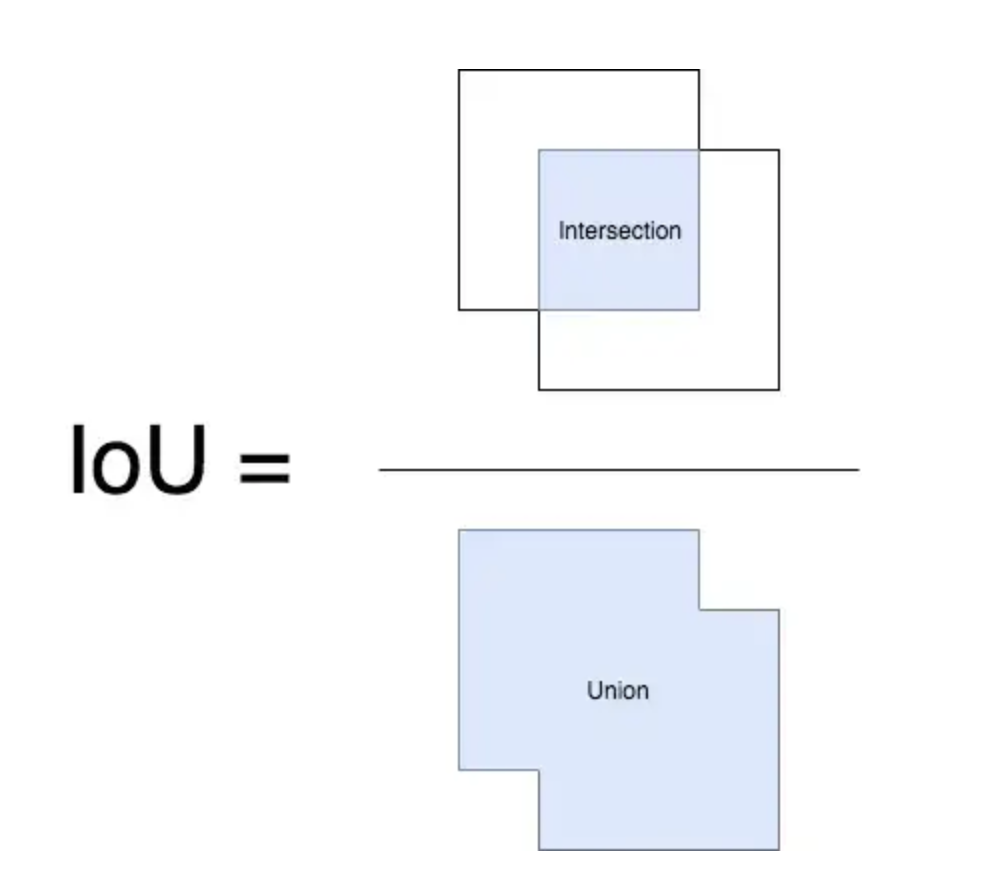
\includegraphics[width=\textwidth]{images/iou.png}}
    \caption{Intersection over Union}
    \label{fig:iou}
\end{figure}
Un score IoU de 1 signifie que la bounding box prédite est parfaitement superposée sur la bounding box réel, tandis qu'un score de 0 signifie qu'il n'y a pas d'air en commun. Idéalement on espère donc avoir un score IoU de 1 pour toutes nos bounding boxes
% -- Joris:


\section{Lecture d'un benchmark COCO}
Un benchmark COCO peut être affiché dans la console comme présenté dans l'image \ref{fig:eval_coco_benchmark}. Ce benchmark est réalisé en suivant l'API COCO\footnote[1]{\url{cocodataset.org/\#detection-eval}}. Il présente deux métrics la précision ($\displaystyle{\frac{TP}{TP+FP} }$) et le rappel ($\displaystyle{ \frac{TP}{TP+FN}}$).
\begin{figure}[h!]
    \centering
    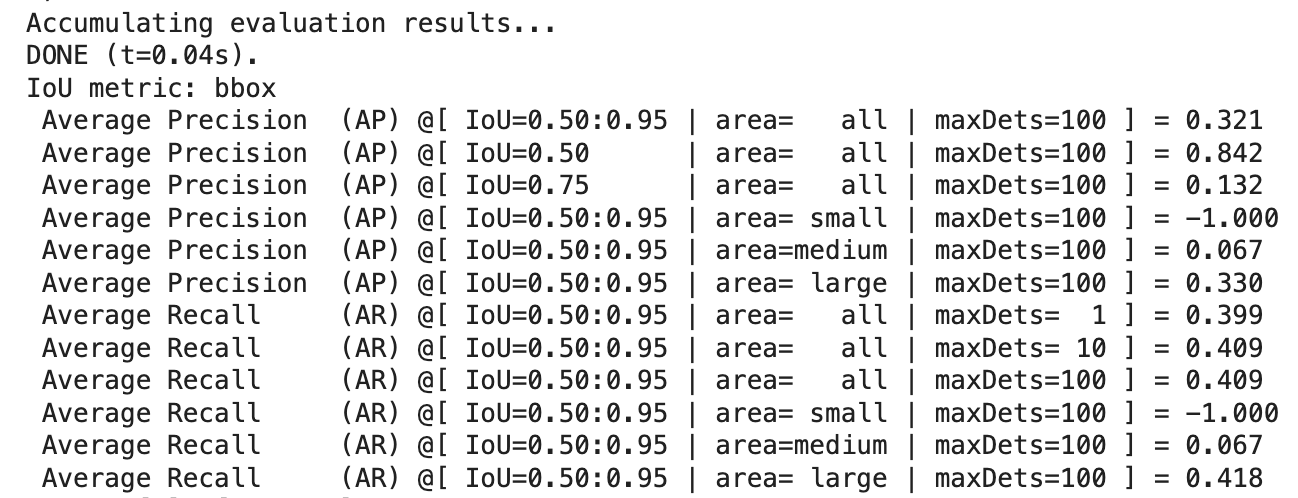
\includegraphics[width=\textwidth]{images/eval_coco_benchmark_white.png}
    \caption{Exemple de benchmark COCO dans la console}
    \label{fig:eval_coco_benchmark}
\end{figure}
La précision moyenne, (AP-Average Precision) présente dans les résultats COCO est calculée sur toutes les catégories, elle correspond traditionnellement au mean Average Precision (mAP).
Les résultats sont divisé en 4 catégories qui dépendent du score IoU ou de l'air de la bounding box prédite.
\begin{itemize}
    \item Les trois premières lignes sont l'AP en considérant différents seuil d'IoU pour sélectionner les boudings boxes à évaluer.
    \item Les trois suivantes sont l'AP en considérant des surfaces de tailles différentes pour sélectionner les boudings boxes à évaluer
    \item Les trois suivantes sont le Rappel Moyens (AR) en considérant plusieurs IoU pour sélectionner les boudings boxes à évaluer.
    \item Les trois suivantes sont l'AR en considérant des surfaces de tailles différentes pour sélectionner les boudings boxes à évaluer.
\end{itemize}
Selon la documentation, la première ligne est la plus importante. A la place de considérer les bounding boxes qui ont un IoU plus grand que le seuil, il est calculé sur cette ligne la moyenne des mAP des bounding boxes selon 10 seuils différents (de 0.5 à 0.95 par pas de 0.05).
%https://github.com/facebookresearch/detectron2/blob/main/MODEL_ZOO.md
Il faut noter que s'il n'existe pas de bounding boxes répondant aux critères, un score de \verb|-1| est affiché. On observe donc qu'il n'existe pas de bounding box de petite taille (32x32 pixels) puisque l'AP ainsi que l'AR où l'air est petite vaut \verb|-1|.
\paragraph{}
Avec Detectron2, un benchmark COCO est fait après chaque époch. C'est à dire lorsque le modèle à vu une fois le dataset en entier. Ce benchmark est effectué sur une fold du set d'entrainement appelé validation. Cependant, afin de véritablement tester les résutlats, nous avons aussi effectué un benchmark COCO sur un set de test d'image jamais vues par le modèle. 
Detectron2 sauvegarde les résultats dans un fichier json, ce fichier peut être lu par un widget TensorBoard afin de monitorer l'entrainement.
Les résultats peuvent aussi être visualisé de manière résumée, par défaut ce n'est pas fait durant l'entrainement uniquement lors d'un benchmark COCO complet. Le résumé s'affiche comme dans l'image \ref{fig:eval_coco_benchmark_resume} 
\begin{figure}
    \centering
    \scalebox{0.5}[0.5]{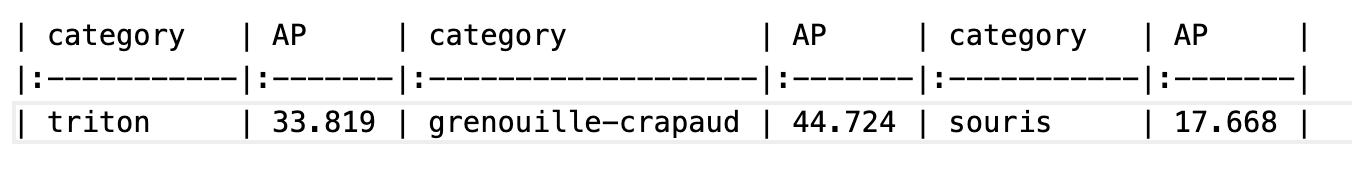
\includegraphics[width=\textwidth]{images/eval_coco_benchmark_resume.png}}
    \caption{Résumé COCO de FASTER RCNN}
    \label{fig:eval_coco_benchmark_resume}
\end{figure}
On voit très facilement que les AP sont désormais calculés par classes sans distinction de IoU. 


\section{ Tensorboard de faster RCNN }
Les widgets tensorboard permettent durant tous les entrainments d'avoir un aperçu des différentes métriques enregistrées nous pouvons donc savoir quand arrêter l'entrainement pour avoir la meilleur performance selon une métrique, cela permet aussi de ne pas overfit. Nous avons pris quelques captures d'écrans affichées dans les figures \ref{fig:tensorboard_overview} et \ref{fig:tensorboard_metric}
\begin{figure}[h!]
    \centering
    \begin{subfigure}[t]{0.49\textwidth}
        \centering
        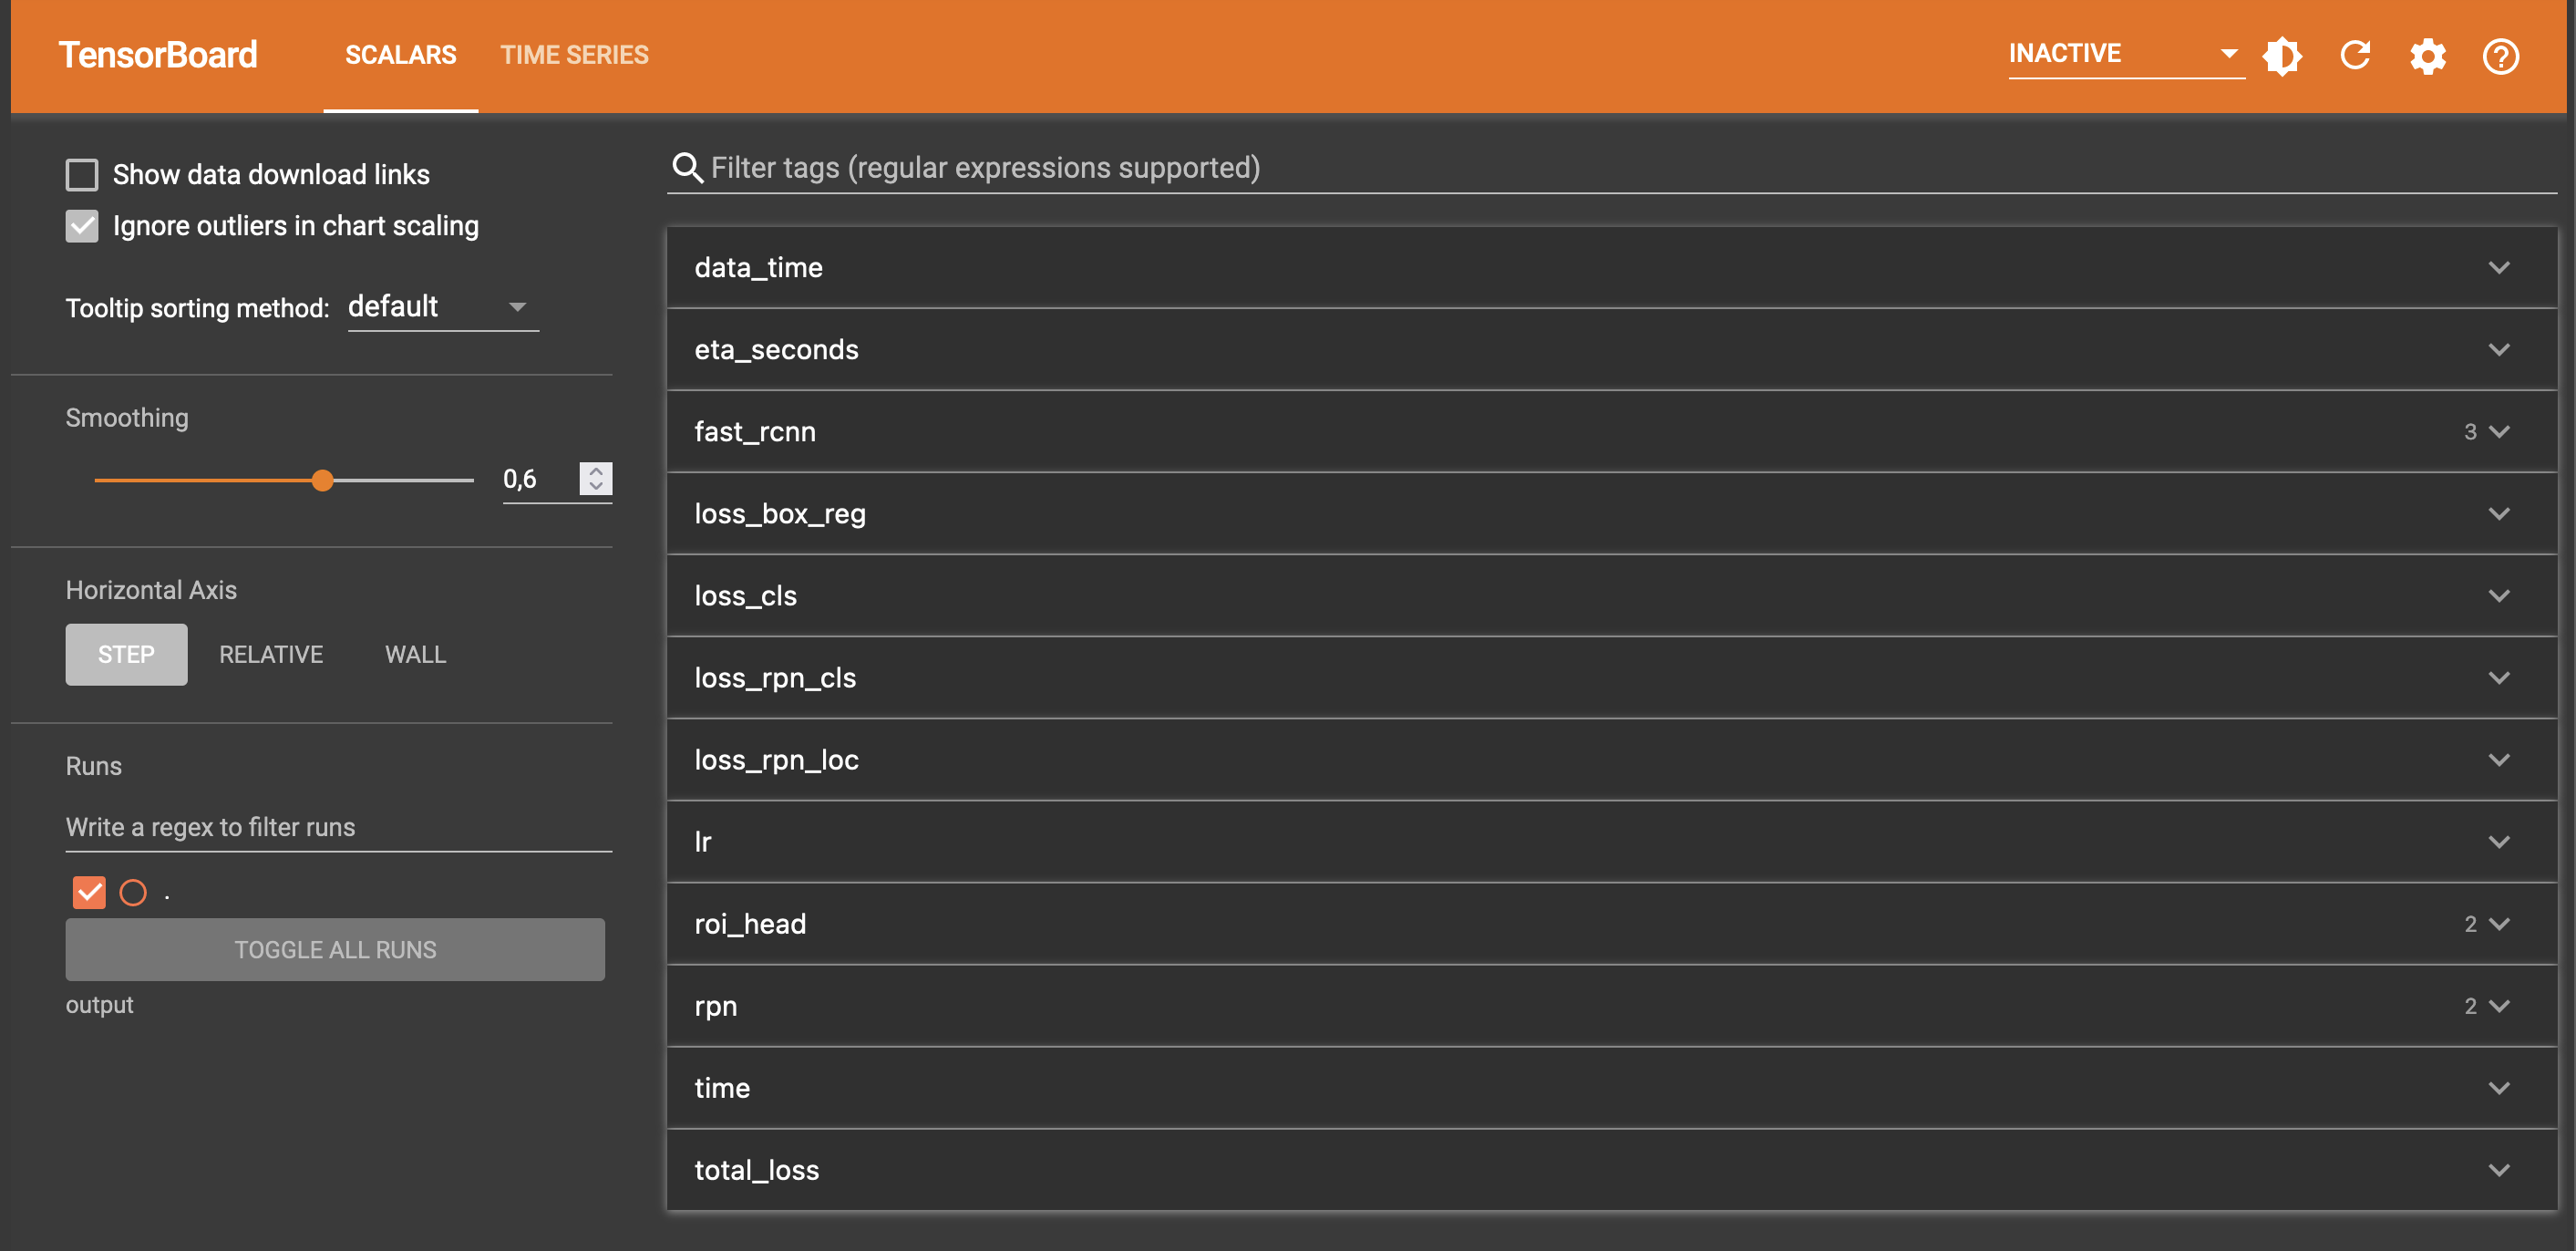
\includegraphics[width=\textwidth]{images/tensorboard_large.png}
        \caption{Aperçu du widget Tensorboard}
        \label{fig:tensorboard_overview}
    \end{subfigure}
    \begin{subfigure}[t]{0.49\textwidth}
        \centering
        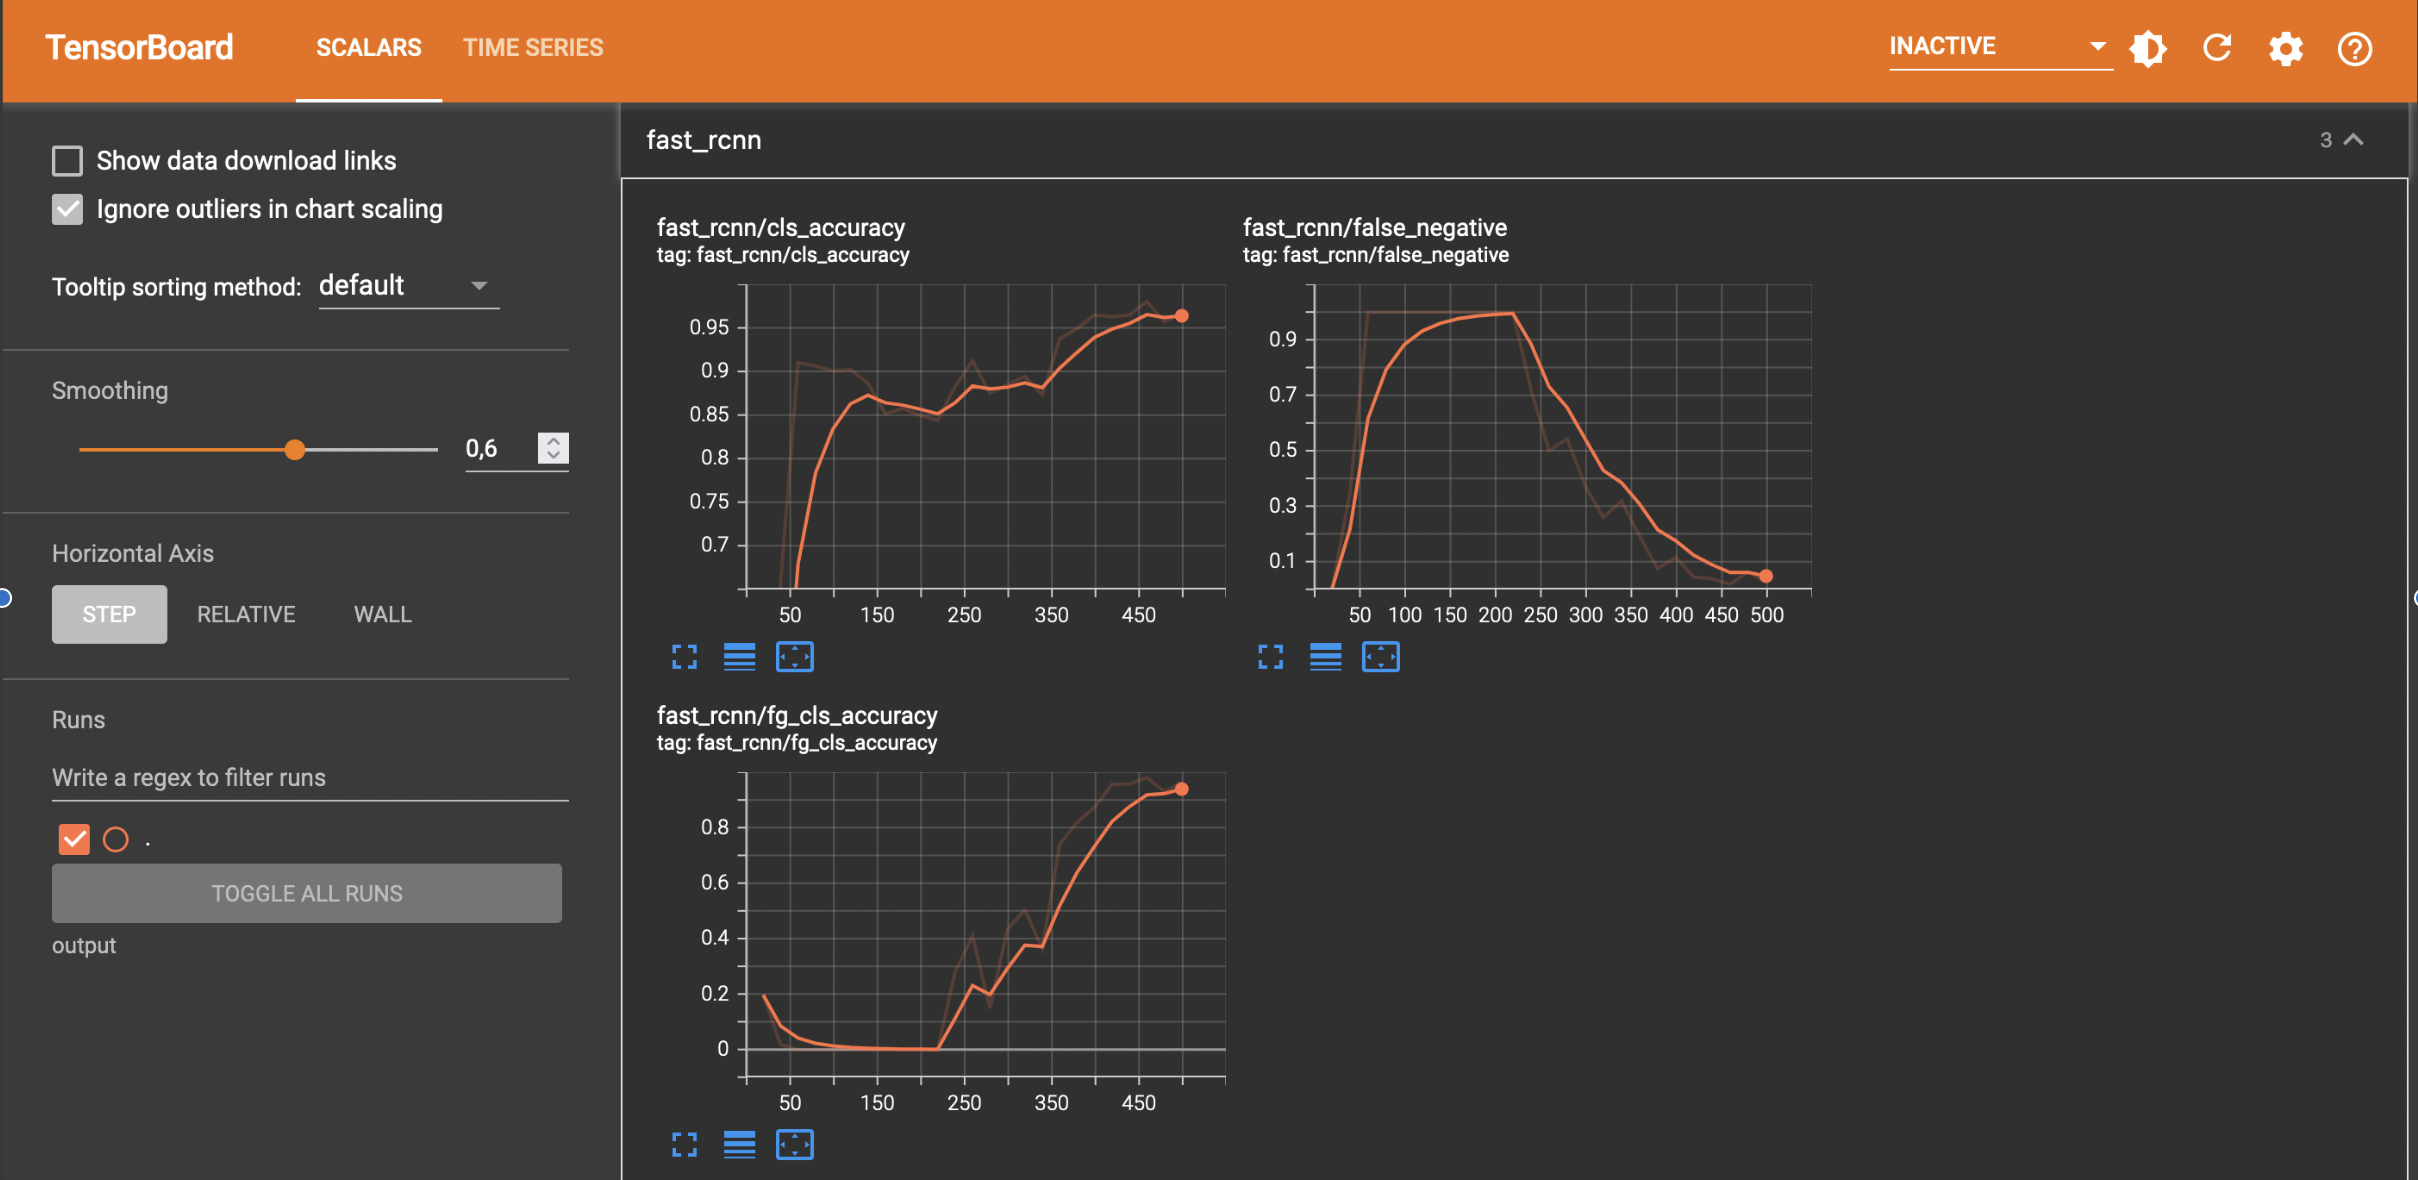
\includegraphics[width=\textwidth]{images/tensorboard_metric.png}
        \caption{Aperçu des métriques enregistrées dans TensorBoard}
        \label{fig:tensorboard_metric}
    \end{subfigure}
    % \scalebox{0.5}[0.5]{}
    % \caption{Aperçu du widget Tensorboard}
    % \label{fig:tensorboard_overview}
    % \scalebox{0.5}[0.5]{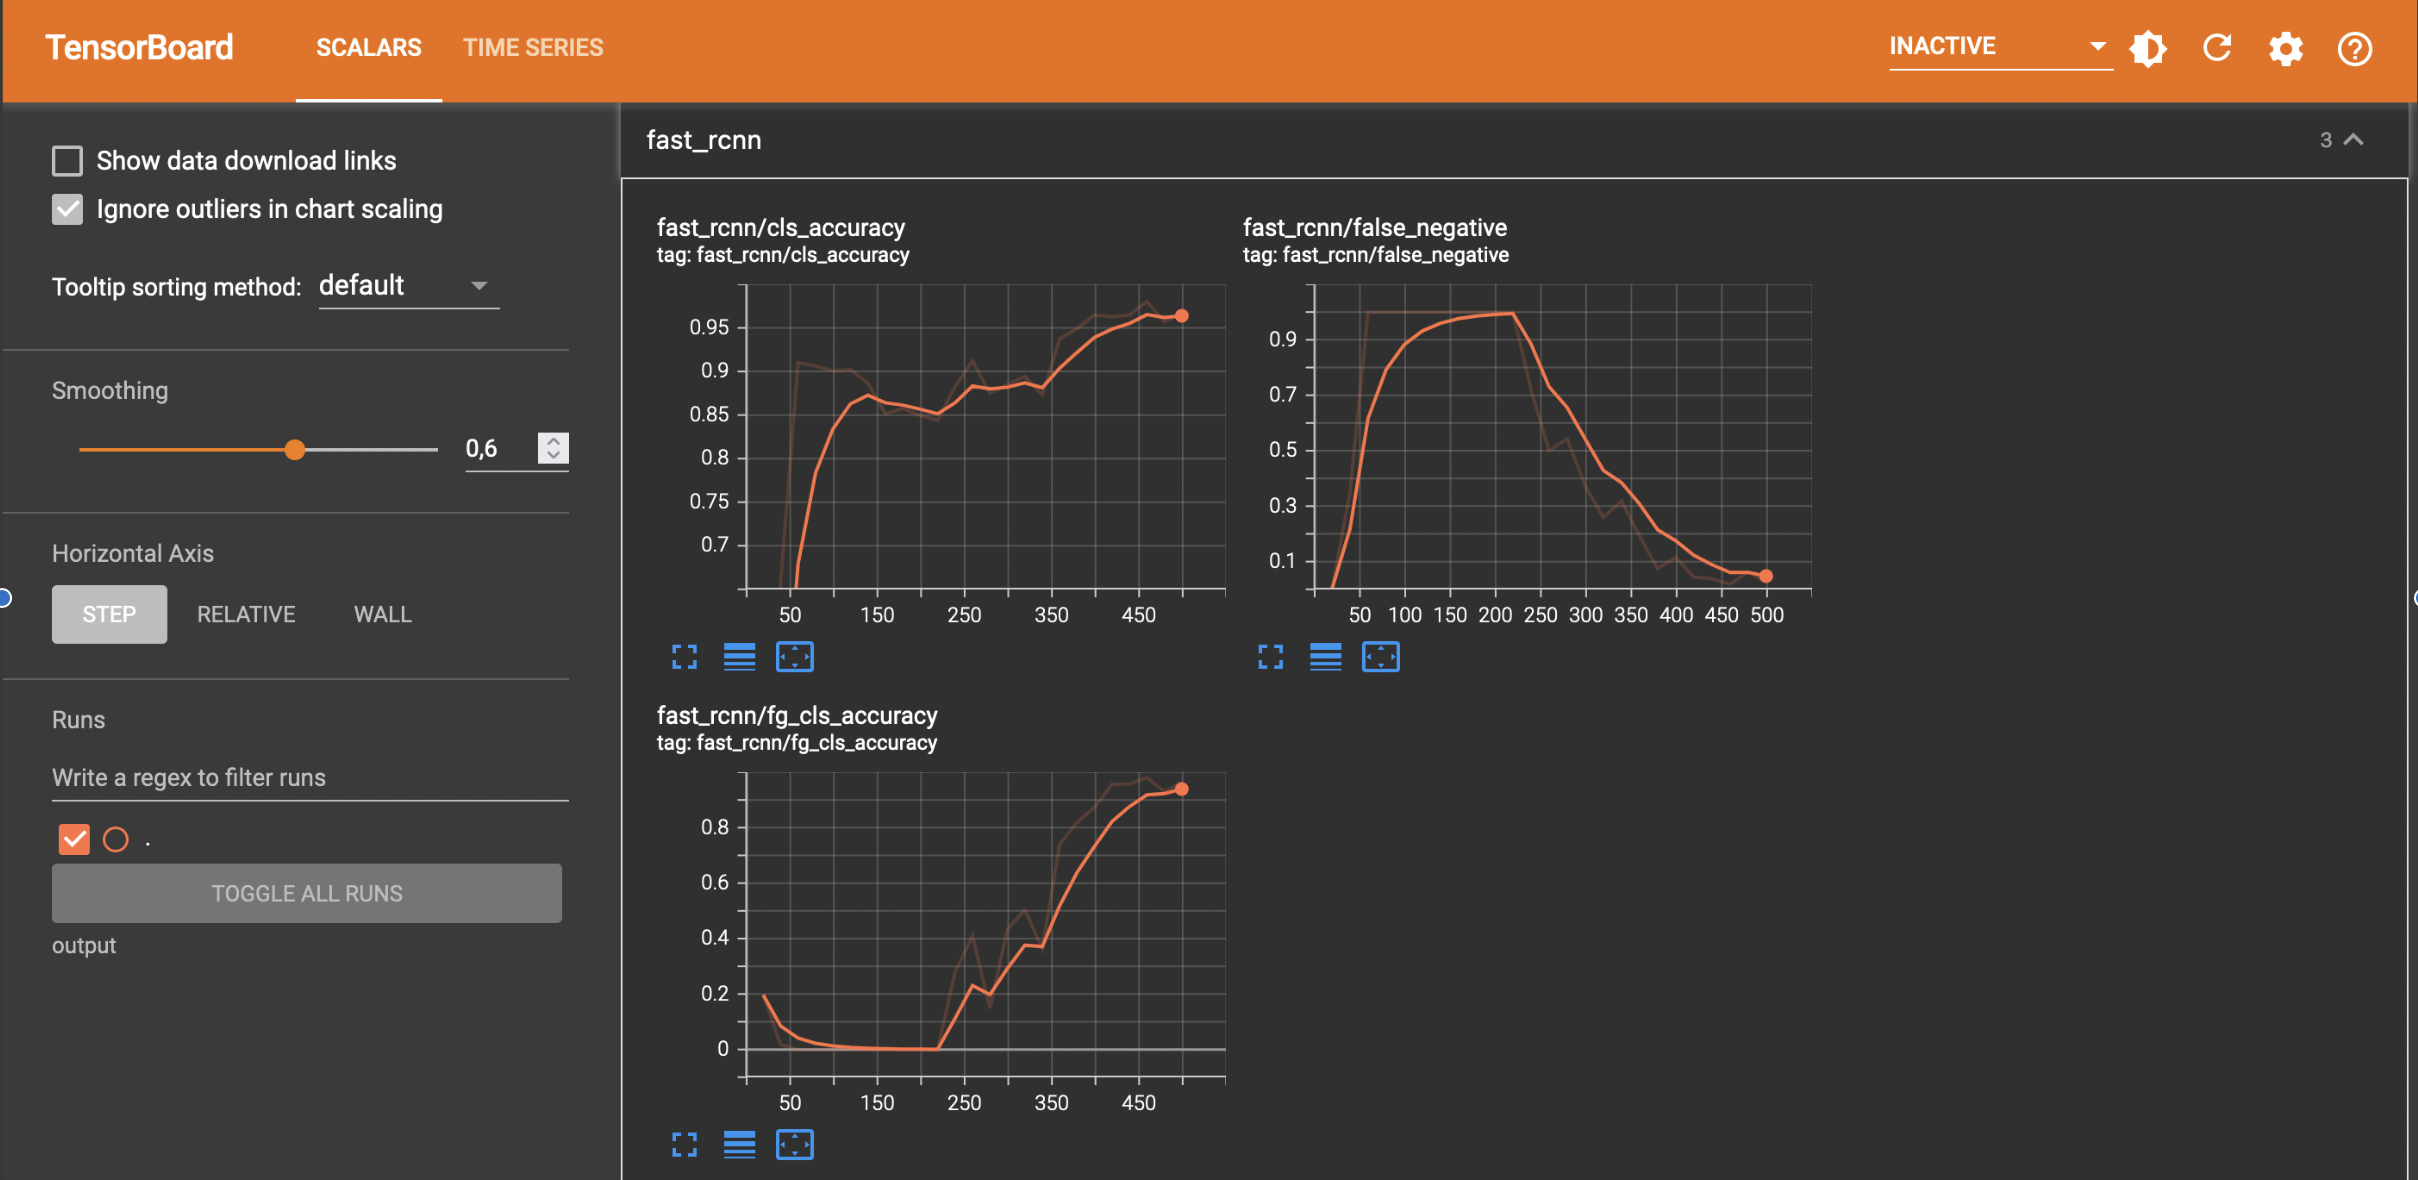
\includegraphics[width=\textwidth]{images/tensorboard_metric.png}}
    % \caption{Aperçu des métriques enregistrées dans TensorBoard}
    \caption{Aperçu de tensorboard et des métriques de faster RCNN}
\end{figure}
Detectron2 affiche aussi une loss total, nous n'avons pas réussis à déterminer la manière dont elle est calculée, mais elle reste un bon indicateur de la performance du model et de l'over/under fitting. De plus comme nous avons plusieurs modèles, nous pouvons les comparer entres eux puisques toutes erreurs sera identiques sur tous les modèles
\begin{figure}[hb!]
    \centering
    \scalebox{0.5}[0.5]{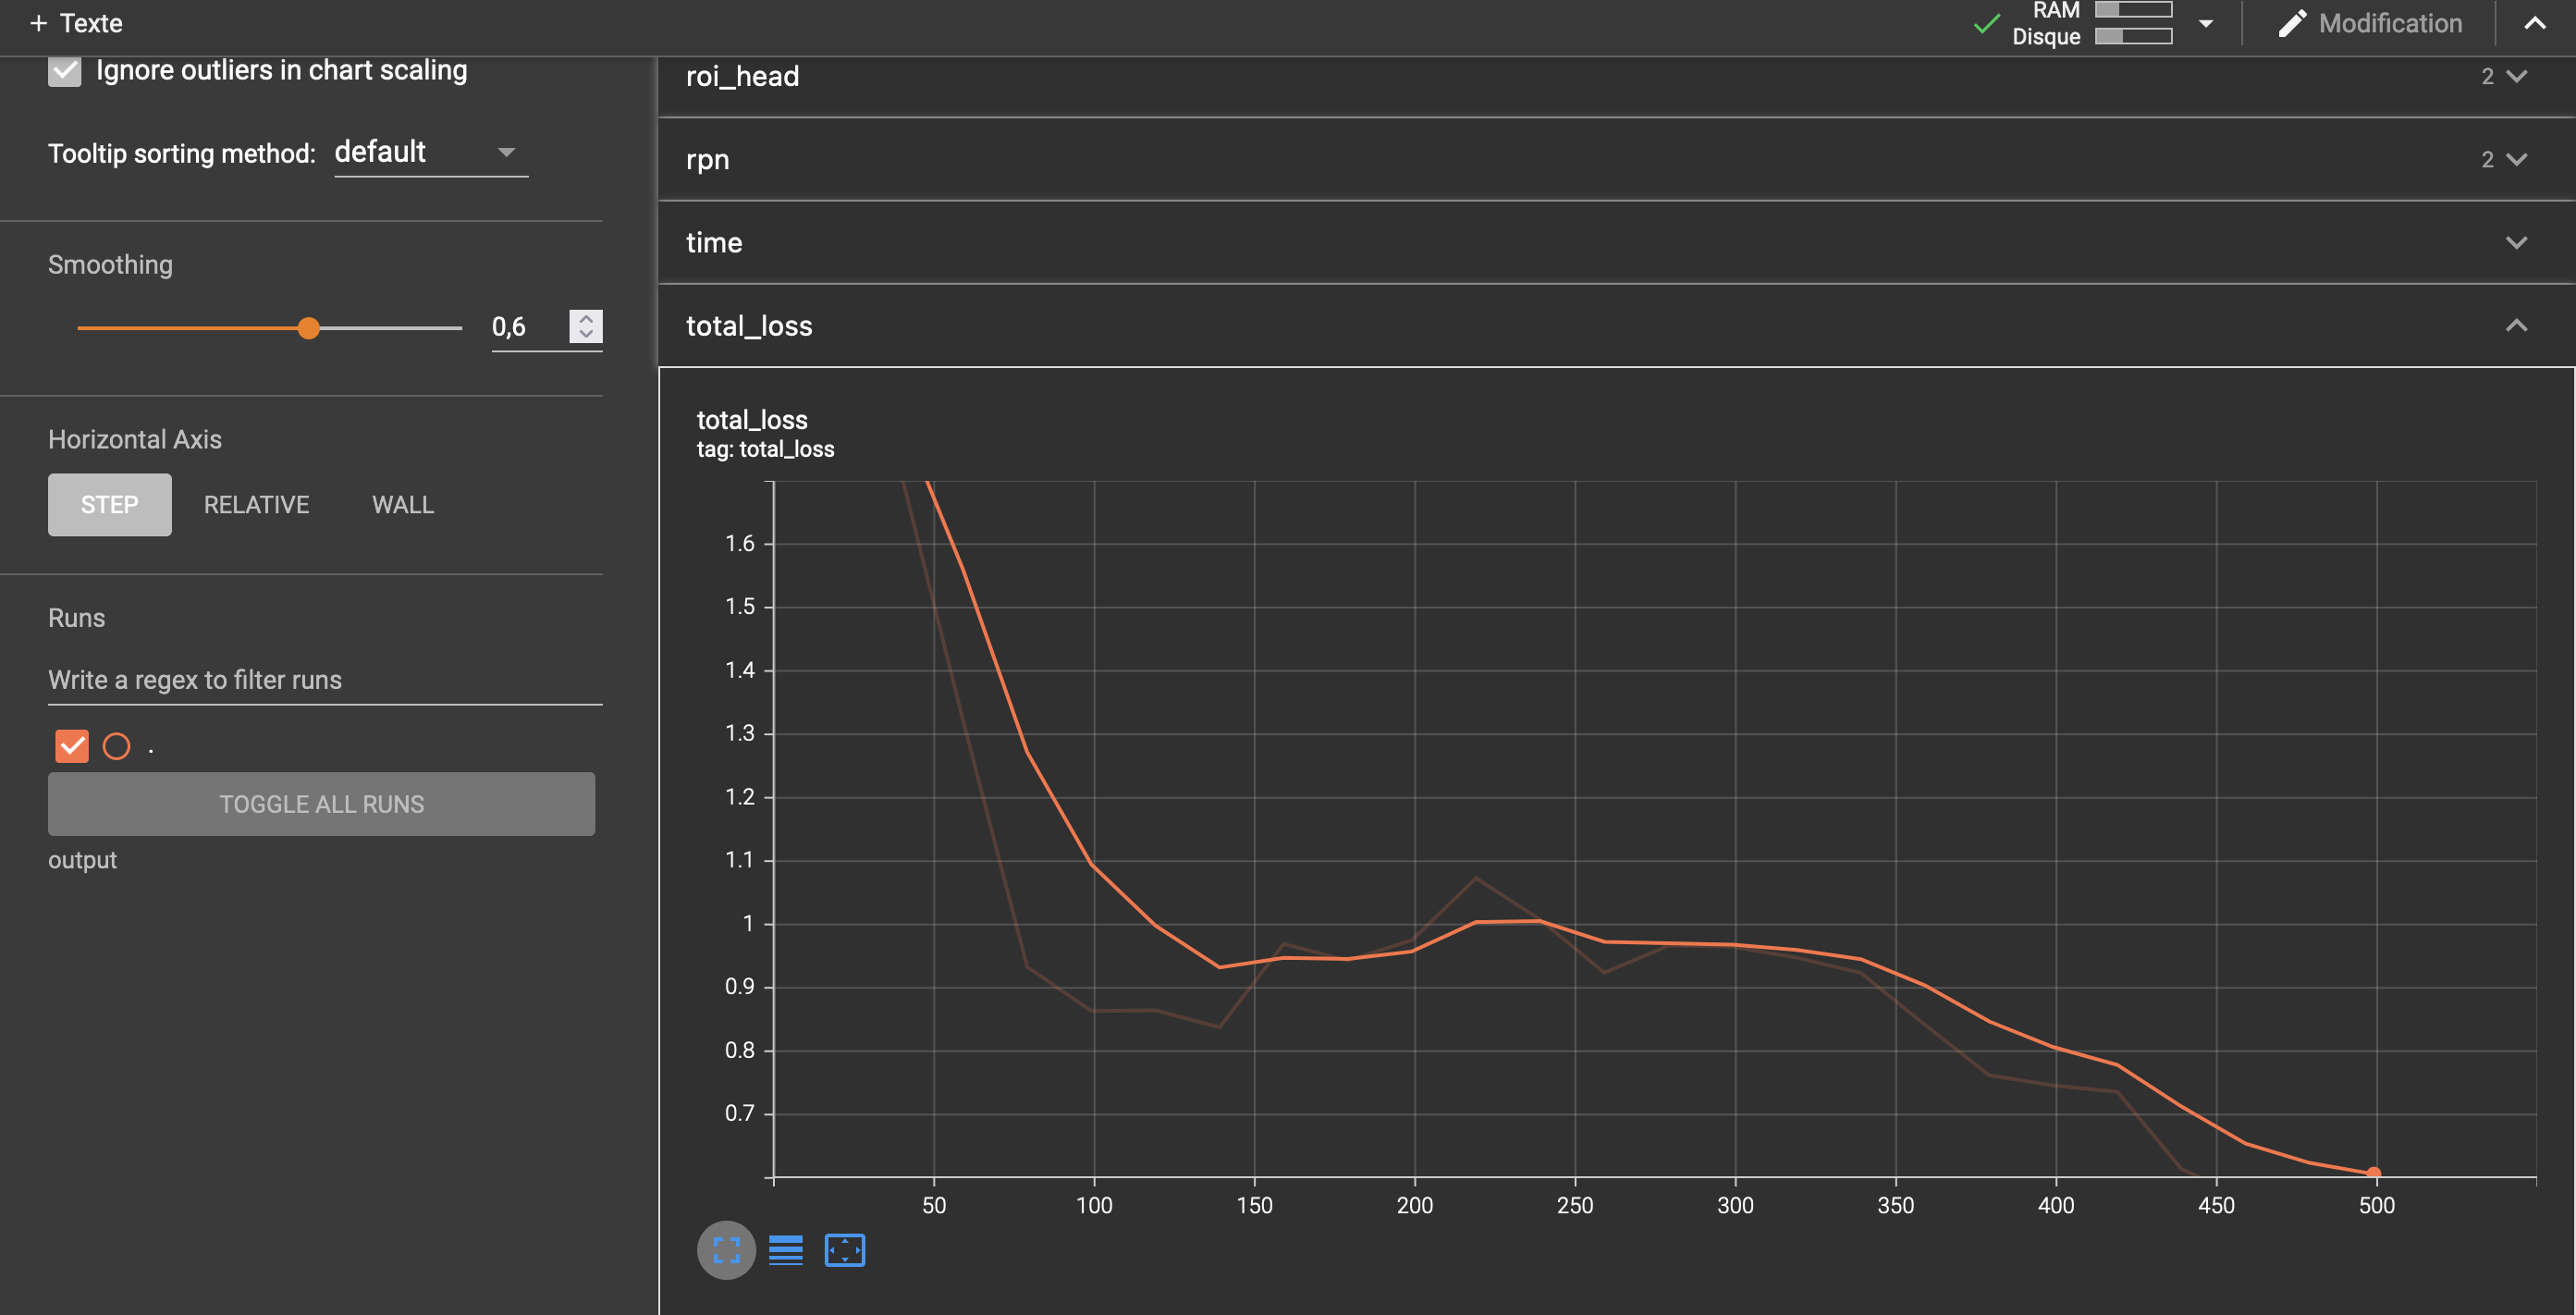
\includegraphics[width=\textwidth]{images/loss_faster_rcnn.png}}
    \caption{Aperçu de la loss total enregistrée dans TensorBoard}
    \label{fig:loss_faster_rcnn}
\end{figure}
Comme nous pouvons le voir dans la figure \ref{fig:loss_faster_rcnn}, nous n'avons ni d'overfit, ni d'underfit.


\section { Loss de RetinaNet}
Dans cette section nous allons observer les métriques du modèle RetinaNet. Ce modèle enregistre moins de métriques, ceci est du au fait qu'il ne possède pas une architecture aussi complexe que Faster-RCNN. Alors que Faster-RCNN présentait des métriques pour certaines parties spécifiques du réseau, les RPN (Region Proposal Network) par exemple, RetinaNet ne présente que deux métriques relatives à l'entrainement : la loss de classification ainsi que la loss des bounding boxes.
\begin{figure}[h!]
    \begin{subfigure}[h]{0.49\textwidth}
        \centering
        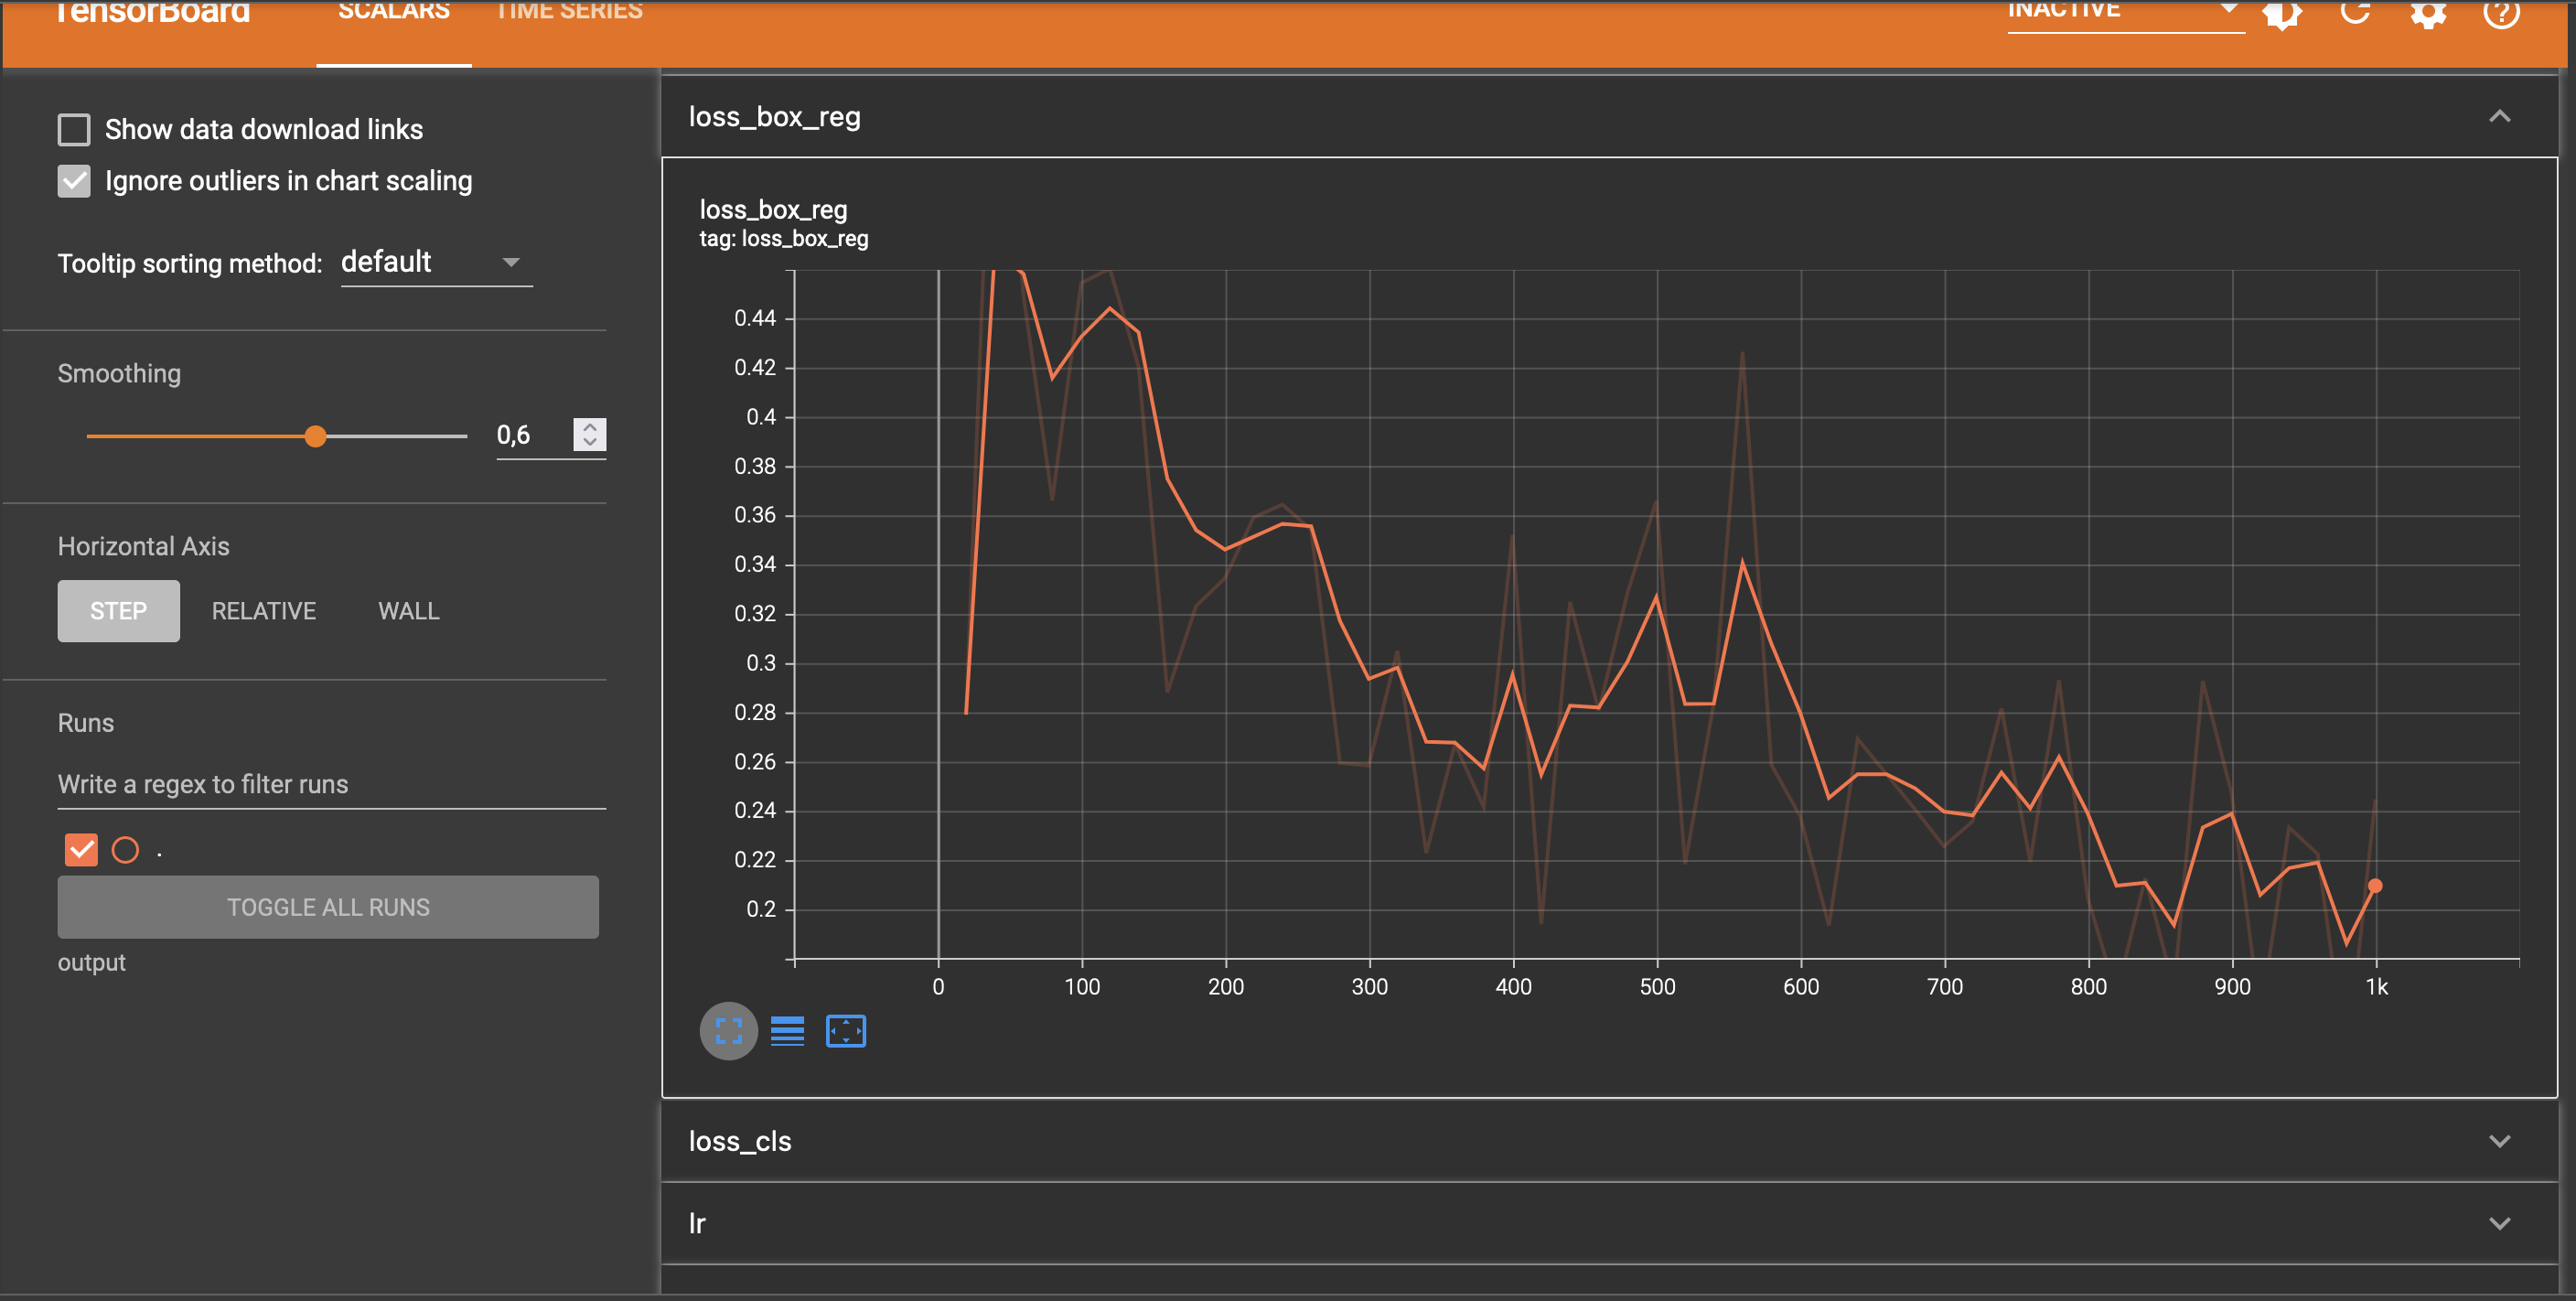
\includegraphics[width=\textwidth]{images/tensorboard_retina_net_loss_box.png}
        \caption{Loss des bounding boxes}
        \label{fig:loss_retinanet_box}
    \end{subfigure}
    \begin{subfigure}[h]{0.49\textwidth}
        \centering
        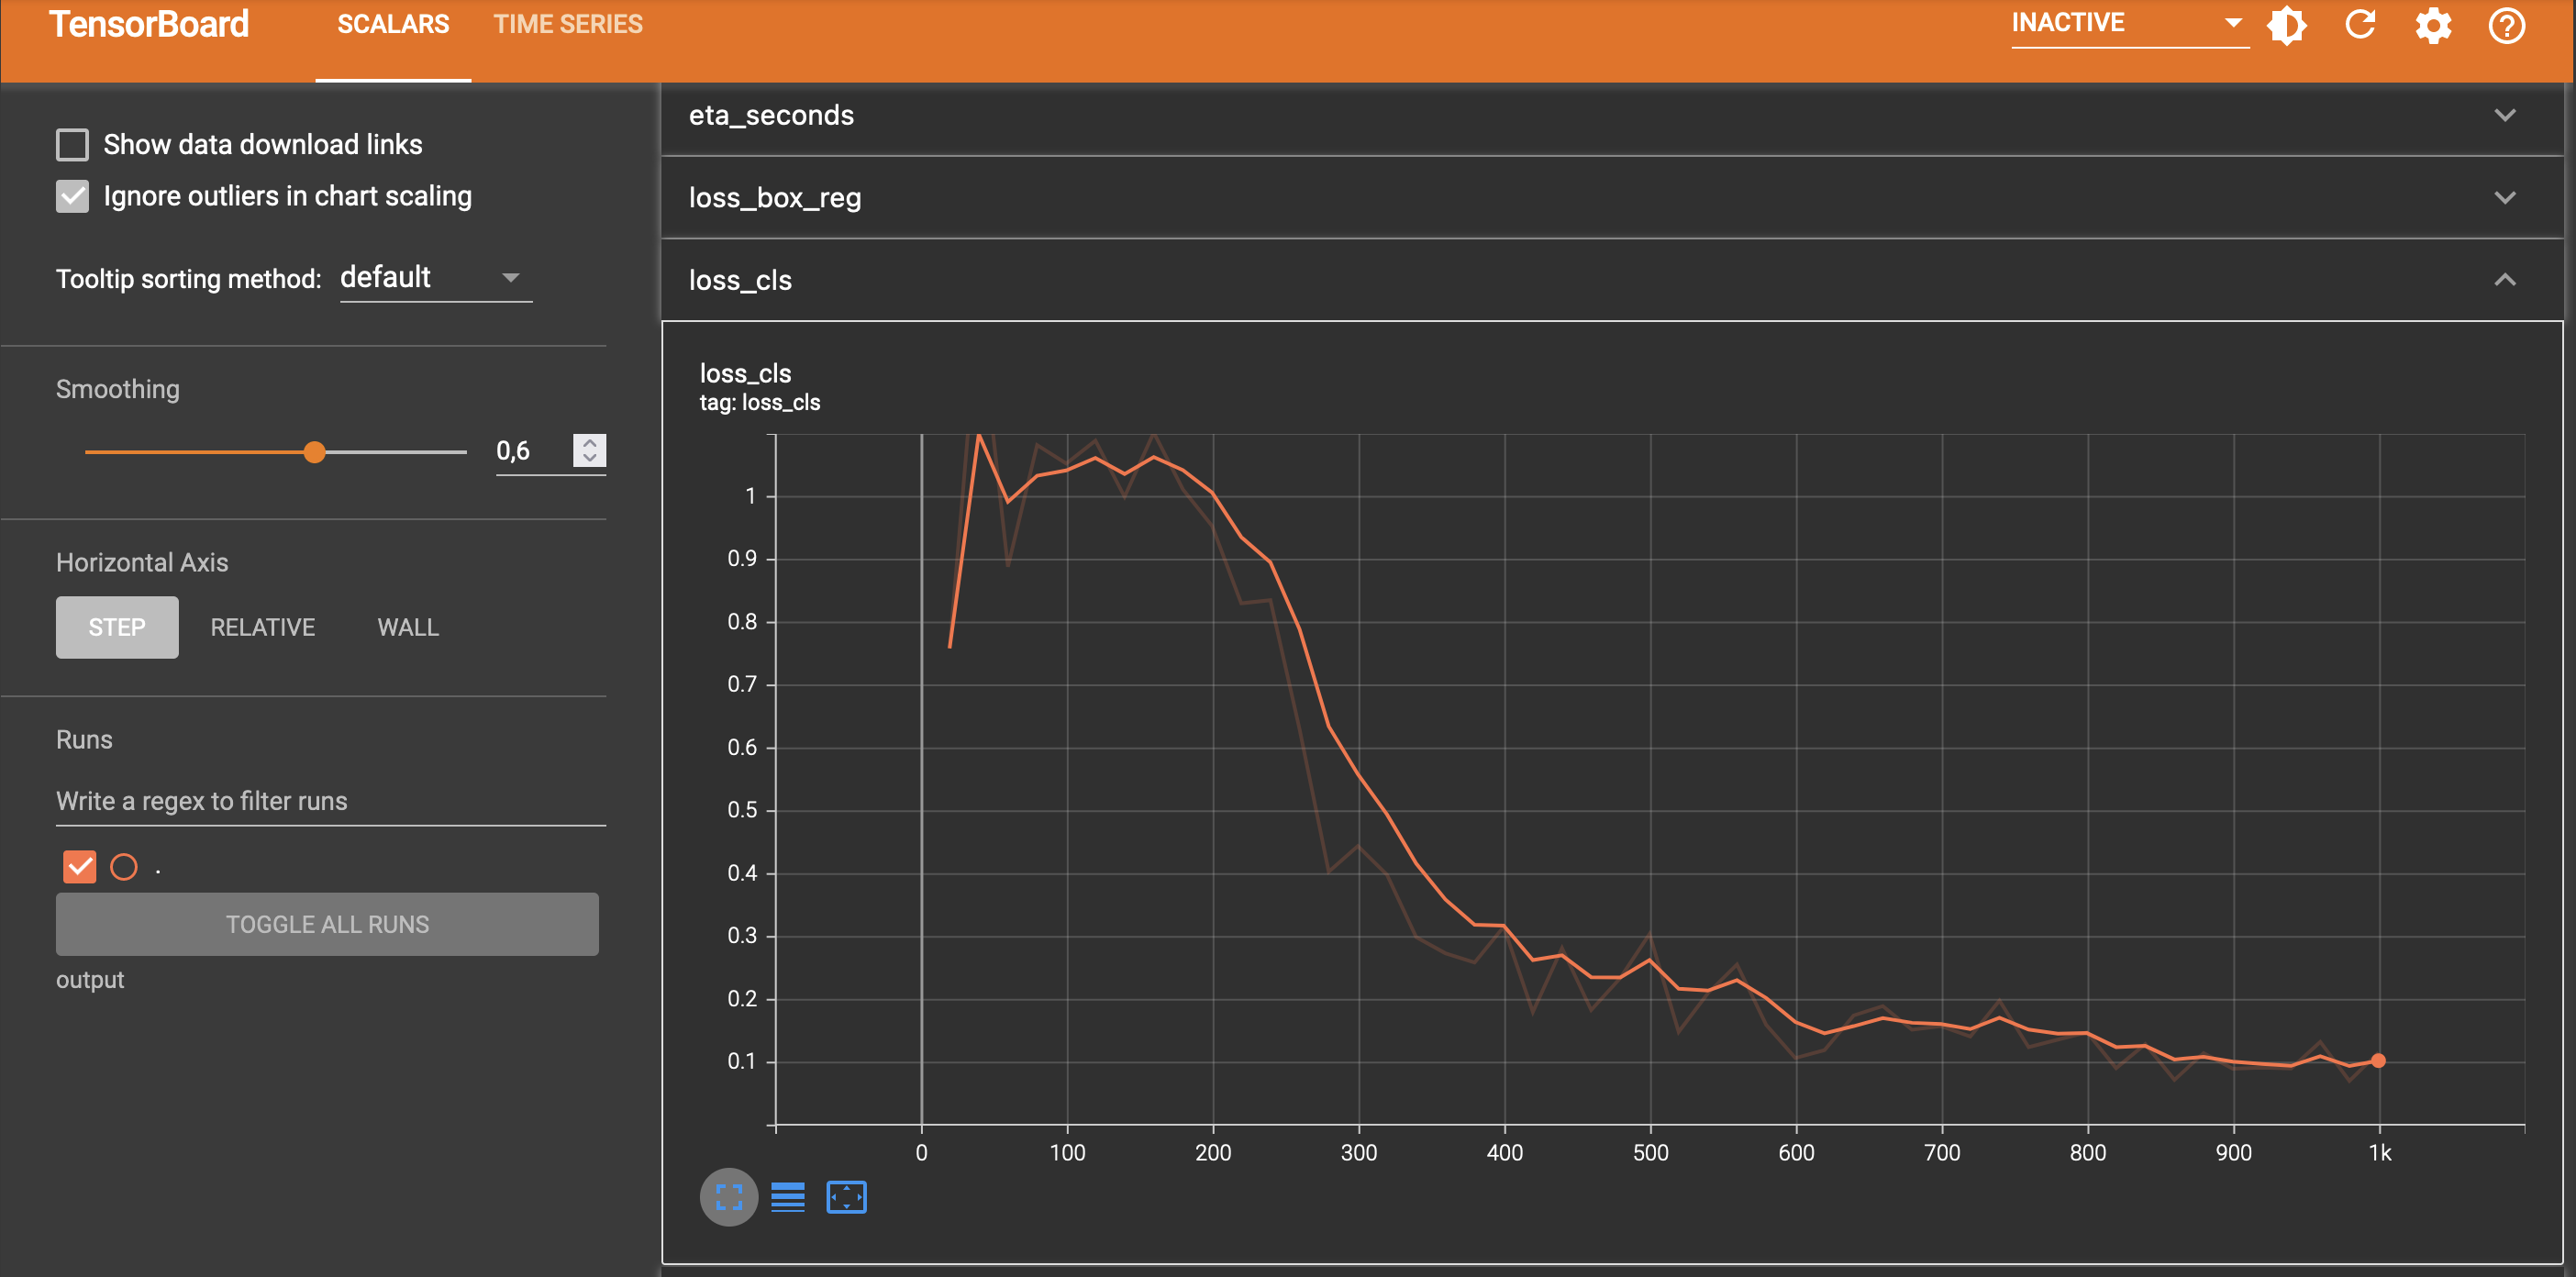
\includegraphics[width=\textwidth]{images/tensorboard_retina_net_loss_cls.png}
        \caption{Loss pour la classification}
        \label{fig:loss_retinanet_cls}
    \end{subfigure}
    \caption{Les métriques de RetinaNet durant un entrainement}
\end{figure}
Nous pouvons observer que RetinaNet doit être plus entrainé, 1000 itérations contre 500 pour Faster-RCNN. Il ne faut pas confondre itérations et époch. Une époch représente un passage sur l'entièreté du dataset, tandis qu'une iteration est pas vers la recherche d'un minimum durant l'optimisation de l'erreur. Nous avons déterminé ces hyperparamètres grâce à tensorboard qui permet durant l'entrainment d'avoir un aperçu des métriques. Fait intéressant, RetinaNet est plus rapide à entrainer (environ 10 minutes de moins que Faster-RCNN) ceci est surement du à son architecture plus simple qui nécessite moins de calcule.

% -- Vic : 

\section{Évaluations des deux modèles sélectionnés}

Après avoir testé plusieurs approches comme mentionnées dans le chapitre \ref{chap:Modeles}, nous avons retenu deux modèles dont nous allons ici comparer les scores d'évaluation :

\begin{itemize}
    \item[-] Faster R-CNN avec Detectron2 et
    \item[-] Retinanet avec Detectron2.
\end{itemize}

Voici donc un tableau résumant les average precision (AP) scores de chaque catégorie suivant le treshold, ainsi 

Scores par classe : 

\begin{center}
   \begin{tabular}{ | l | l || c |}
     \hline
     modèle & catégorie & AP score \\ \hline
     \multirow{2}{*} {Faster R-CNN} & crapaud-grenouille & 42.03 \\ 
     & triton & 42.58   \\ \hline
     \multirow{2}{*} {Retinanet} & crapaud-grenouille & 49.40 \\
    & triton & 0.00 \\
     \hline
   \end{tabular}
 \end{center}

 Bien que le score pour la classe crapaud-grenouille soit plus élevé à l'aide du modèle Retinanet, le score pour la classe triton est de zéro. Rappelons que la tâche initiale de ce projet est de compter le nombre de triton/crapaud-grenouille qui utilisent les crapauduc ; ainsi, nous avons choisi l'algorithme Faster R-CNN comme modèle final pour cette tâche de classification.

\subsection{Modèle final choisi}

\paragraph{Entraînement}

Voici donc comment nous avons premièrement entraîné notre modèle Faster R-CNN, avec Detectron 2 : 

\lstset{language=Python}
\begin{lstlisting}
cfg = get_cfg()
cfg.merge_from_file(model_zoo.get_config_file("COCO-Detection/
faster_rcnn_X_101_32x8d_FPN_3x.yaml"))
cfg.DATASETS.TRAIN = ("triton_train",)
cfg.DATASETS.TEST = ()
cfg.DATALOADER.NUM_WORKERS = 2
cfg.MODEL.WEIGHTS = model_zoo.get_checkpoint_url("COCO-Detection/
faster_rcnn_X_101_32x8d_FPN_3x.yaml")  
cfg.SOLVER.IMS_PER_BATCH = 2 
cfg.SOLVER.BASE_LR = 0.00020 
cfg.SOLVER.MAX_ITER = 500 
cfg.SOLVER.STEPS = []   
cfg.MODEL.ROI_HEADS.BATCH_SIZE_PER_IMAGE = 128  
cfg.MODEL.ROI_HEADS.NUM_CLASSES = 4 
\end{lstlisting}


\paragraph{Test}

Et voici donc le modèle construit pour tester nos données d'évaluation : 

\lstset{language=Python}
\begin{lstlisting}
# on recuperation des poids du modele qu'on vient d'entrainer
cfg.MODEL.WEIGHTS = os.path.join(cfg.OUTPUT_DIR, "model_final.pth")  
# determination d'un treshold pour le test
cfg.MODEL.ROI_HEADS.SCORE_THRESH_TEST = 0.7  
# construction du predicteur
predictor = DefaultPredictor(cfg)
\end{lstlisting}

Le treshold choisi pour le test ci-dessus indique donc qu'on considérera une image comme étant prédite d'une certaine classe si le modèle est sûr à au moins 70\% de sa classification.\newline

Voici deux exemples de résultats de classification par notre modèle ainsi créé :

\begin{figure}[H]
    \centering
    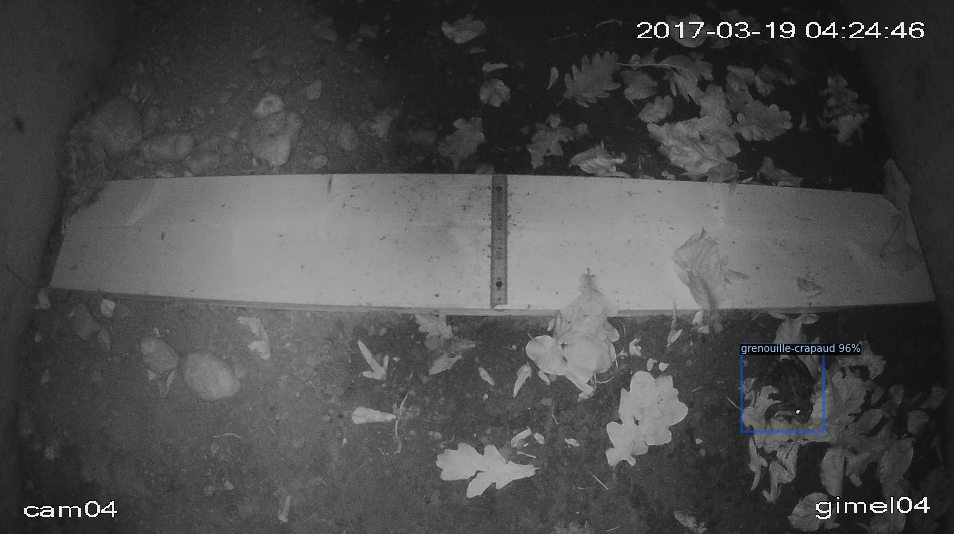
\includegraphics[width=300px]{images/Eval_FasterRCNN_crapGren.png}
    \caption{Prédiction de Faster R-CNN - crapaud-grenouille}
    \label{fig:fasterRcnn_crapGren}
\end{figure}

\begin{figure}[H]
    \centering
    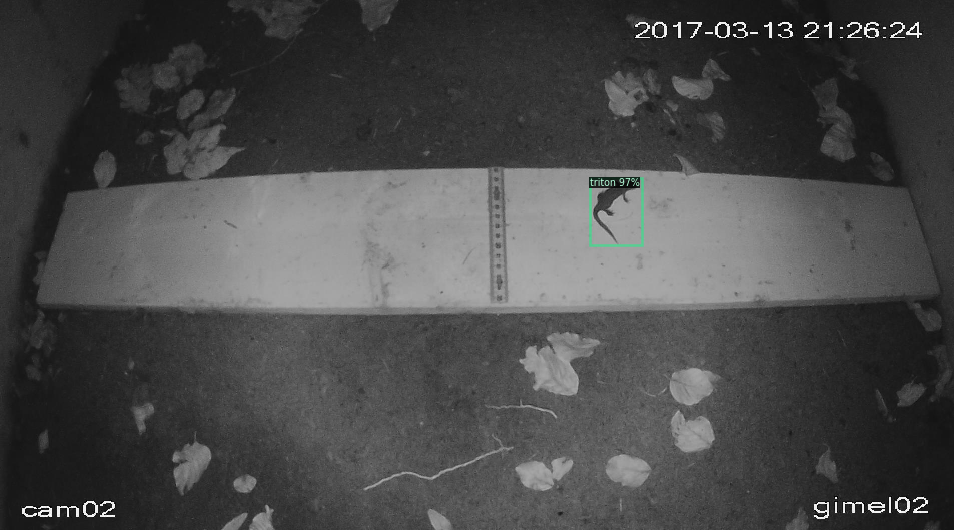
\includegraphics[width=300px]{images/Eval_FasterRCNN_triton.png}
    \caption{Prédiction de Faster R-CNN - triton}
    \label{fig:fasterRcnn_triton}
\end{figure}

Validation (résultats) important de dire que images sont similaires à celles deja vues blabla --> Joris (précision sur ce qui est dit..)

